\chapter{Brugermanual}

I dette afsnit vil vi beskrive en simpel brugermanual til spillet. Vi vil fokusere på den primære styringsmetode vha. rattet og gearstangen. Spillet kan dog også spillet vha. computerens keyboard eller knapperne på udviklings boardet.
\\

Det første der møder en når man starter spillet er skærmbilledet der ses på figur \ref{fig:startup}. Den blinkende tekst under logoet angiver at brugeren skal trykke på en valgfri tast for at starte spillet. ASCII arten af rattet skulle gerne give en indikation af hvordan spillet styres. Et billede af rattet til sammenligning kan ses i figur \ref{fig:rat_med_controls}.

\begin{figure}[h!]
\begin{minipage}[b]{0.49\textwidth}
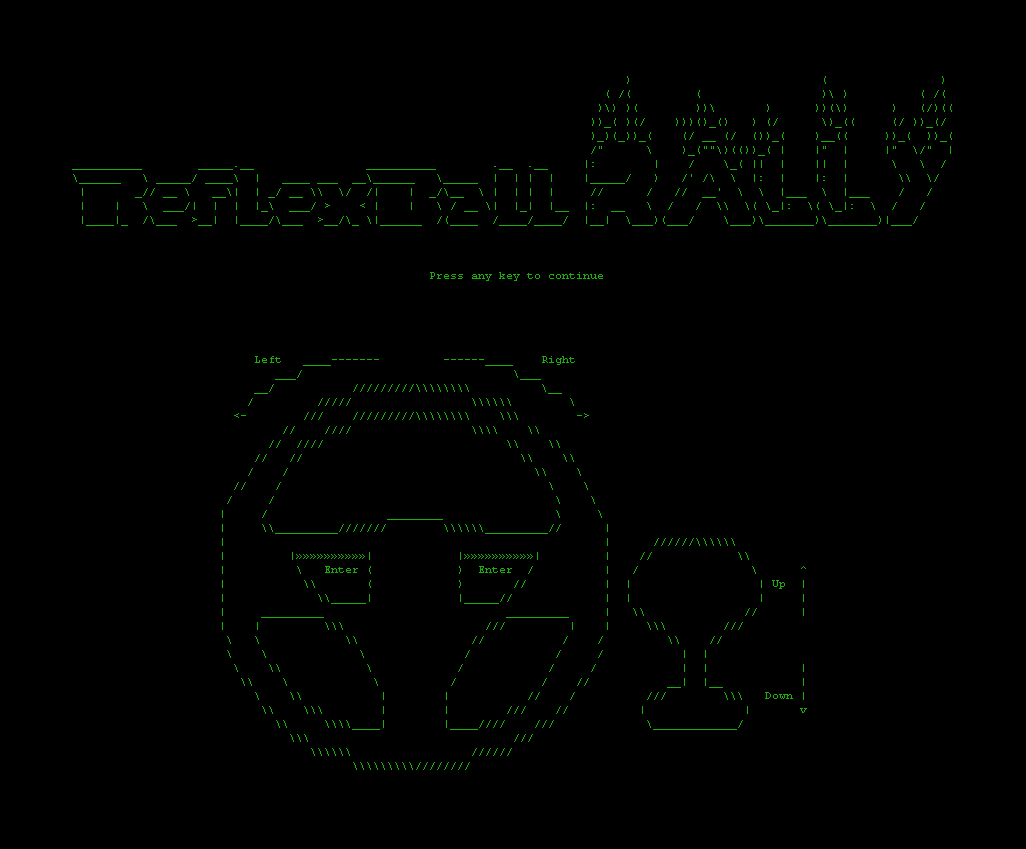
\includegraphics[width=\linewidth]{figs/screenshots/startup_crop.png}
\caption{Screenshot af startup skærmen}
\label{fig:startup}
\end{minipage}\hfill
\begin{minipage}[b]{0.49\textwidth}
\includegraphics[width=\linewidth]{figs/rat_med_controls.png}
\caption{Oversigt over hvordan rattet bruges}
\label{fig:rat_med_controls}
\end{minipage}\hfill
\end{figure}

Derefter vises menuen svarende til den i figur \ref{fig:menu_2}. Her kan brugeren vælge sværhedsgraden. Brugeren kan således flytte bolden op og ned vha. gearet. Når den ønskede sværhedsgrad er valgt kan denne vælges ved at trykke på en af de to knapper der sidder på rattet. Den valgte sværhedsgrad bestemmer derefter bredden af strikeren, samt hvor hurtigt bolden skal begynde at forøge dens hastighed. Ved valg af Chuck Norris mode er boldens hastighed dog den maksimale hastighed fra starten. For mere information henvises til funktionen \nameref{asciidisplay} i appendiks \ref{C kode}. \\

\begin{figure}[h!]
\centering
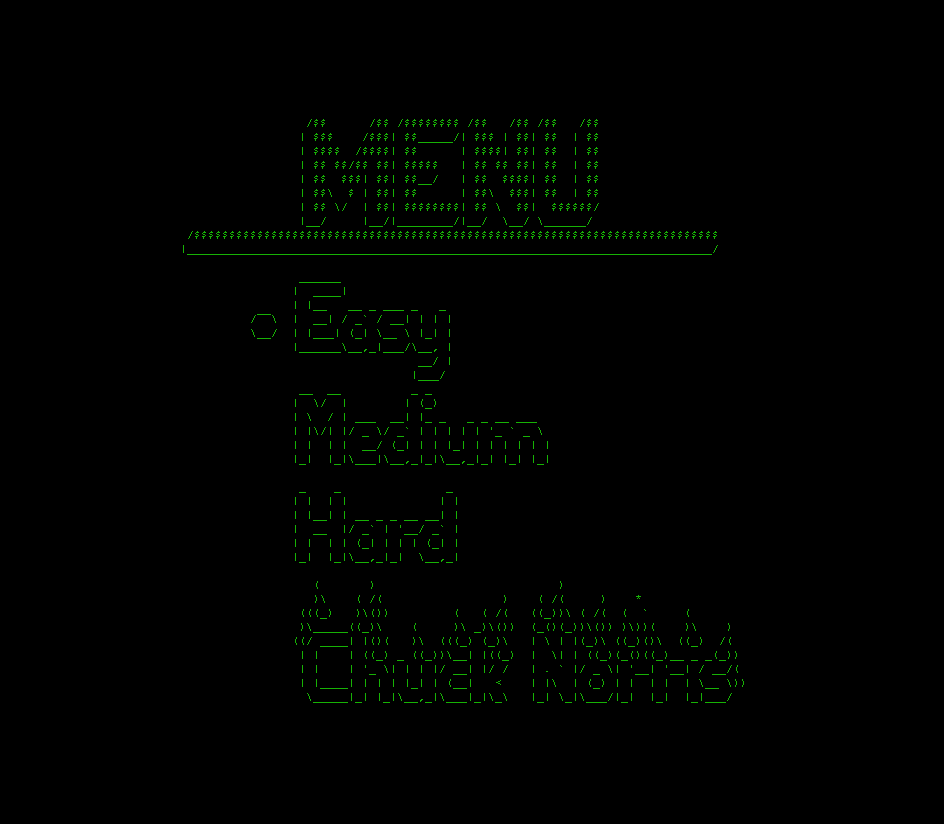
\includegraphics[scale=0.25]{figs/screenshots/menu_crop.png}
\caption{Screenshot af menuen}
\label{fig:menu_2}
\end{figure}

Efter dette begynder selve spillet. Man skyder bolden afsted ved enten af at hive gearet tilbage eller trykke på en af de to knapper på rattet. Bolden vil da skydes afsted med en vinkel på 45-135 grader. Herefter gælder det blot om at skyde alle brikkerne ned ved at bevæge strikeren ved at dreje på rattet. Hvis brugeren skyder alle brikkerne i stykker avancerer brugeren til næste level. \\

Et overblik over alle de 6 levels i spillet kan ses på figurerne nedenfor. Bemærk at der i level 6 er en række usynlige brikker, der først kommer frem når man har ramt dem én gang. Se \nameref{levels} i appendiks \ref{C kode}. \\

\begin{figure}[h!]
\begin{minipage}[b]{0.32\textwidth}
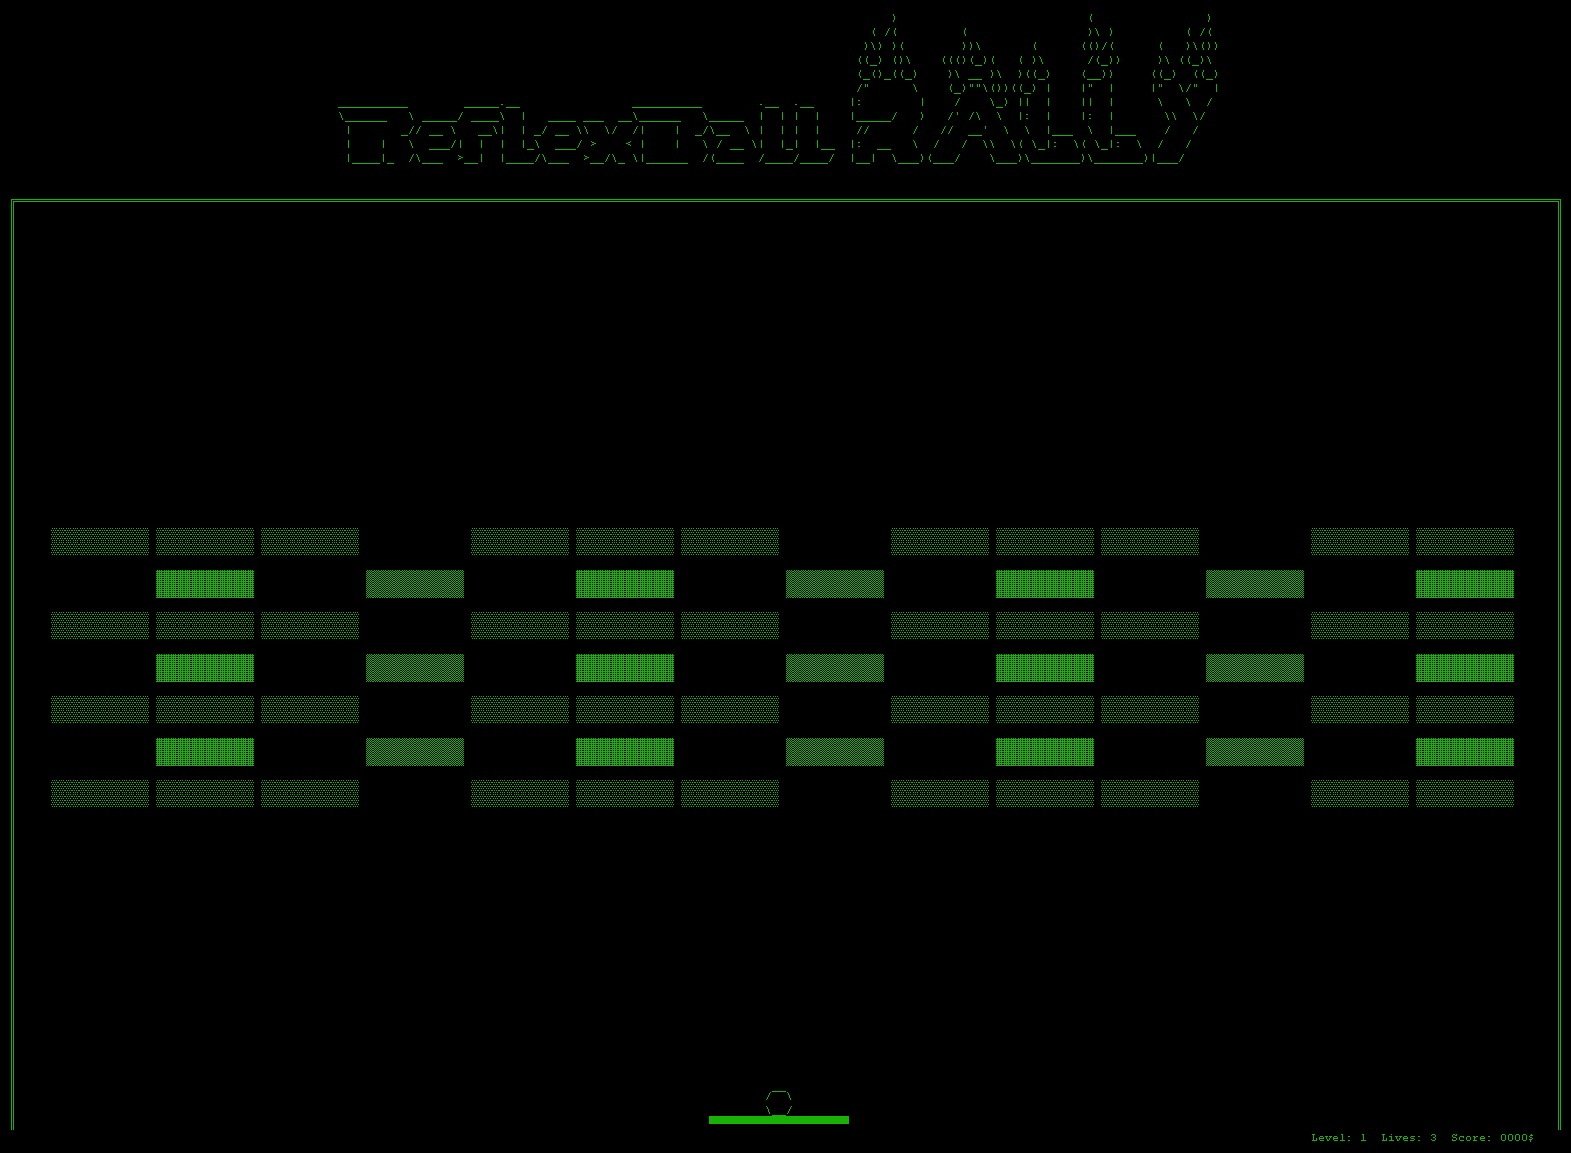
\includegraphics[width=\linewidth]{figs/screenshots/level1.png}
\caption{Level 1}
\label{fig:level1_2}
\end{minipage}\hfill
\begin{minipage}[b]{0.32\textwidth}
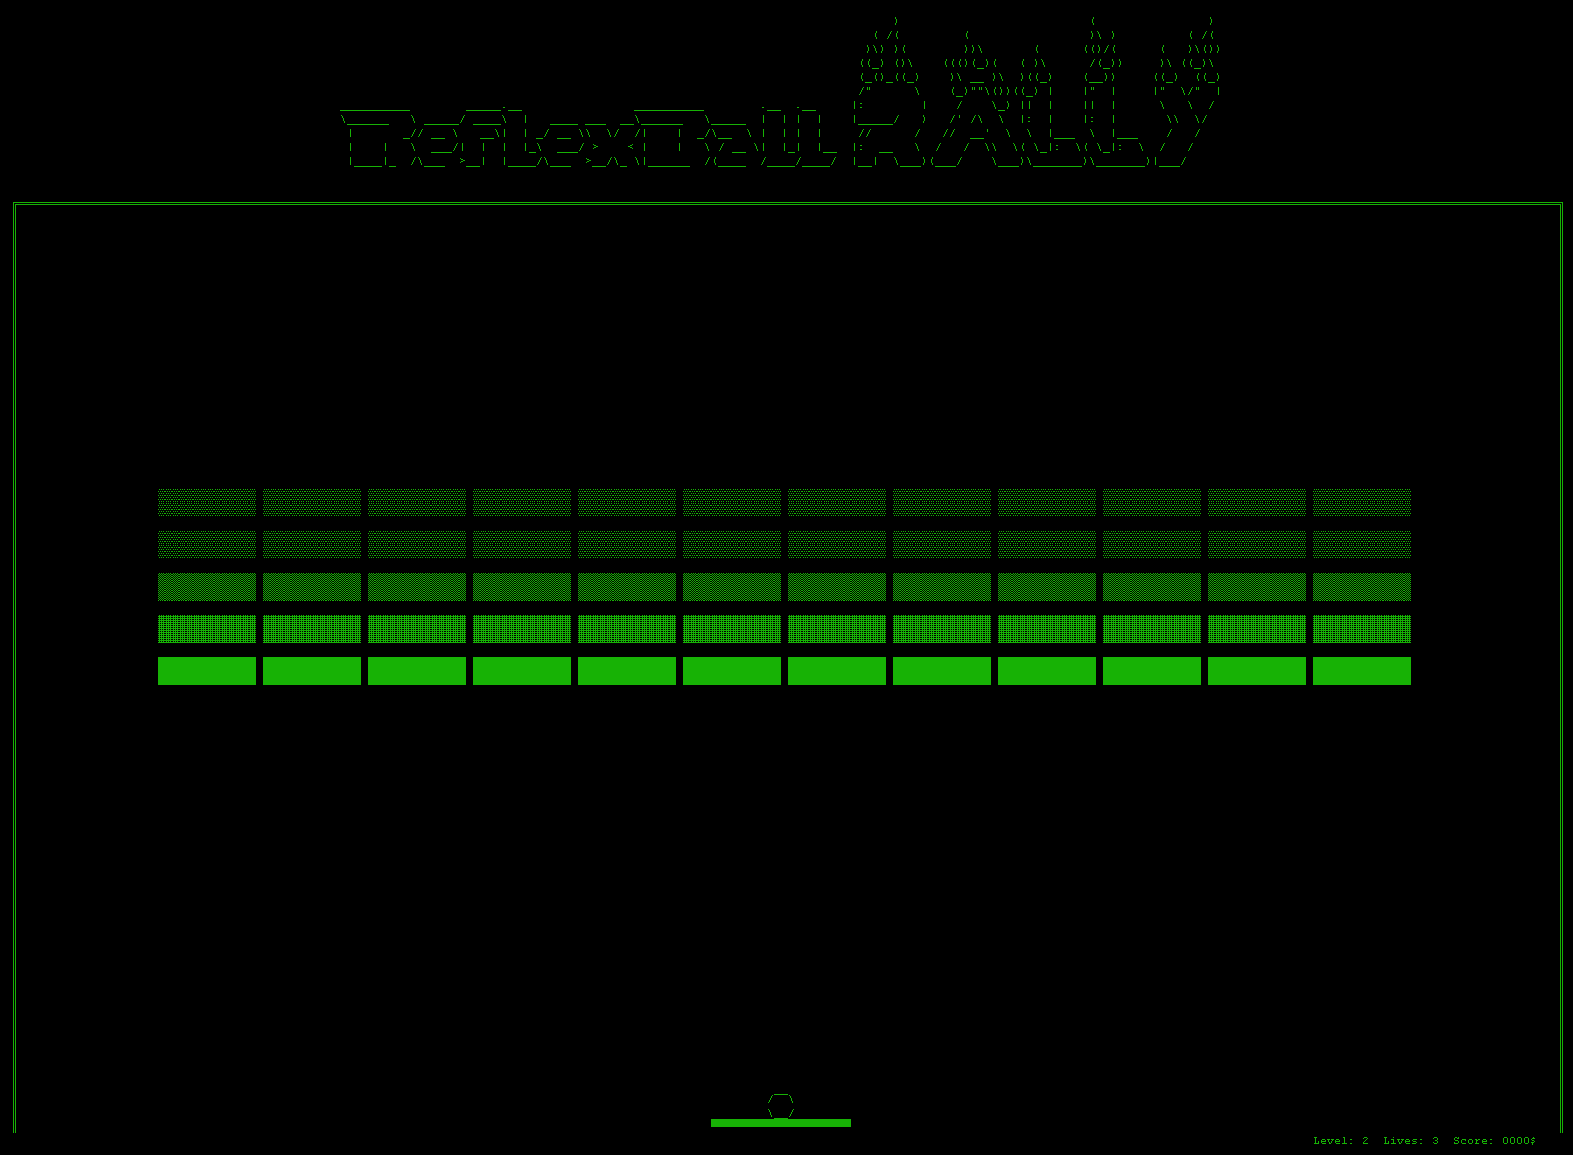
\includegraphics[width=\linewidth]{figs/screenshots/level2.png}
\caption{Level 2}
\label{fig:level2}
\end{minipage}\hfill
\begin{minipage}[b]{0.32\textwidth}
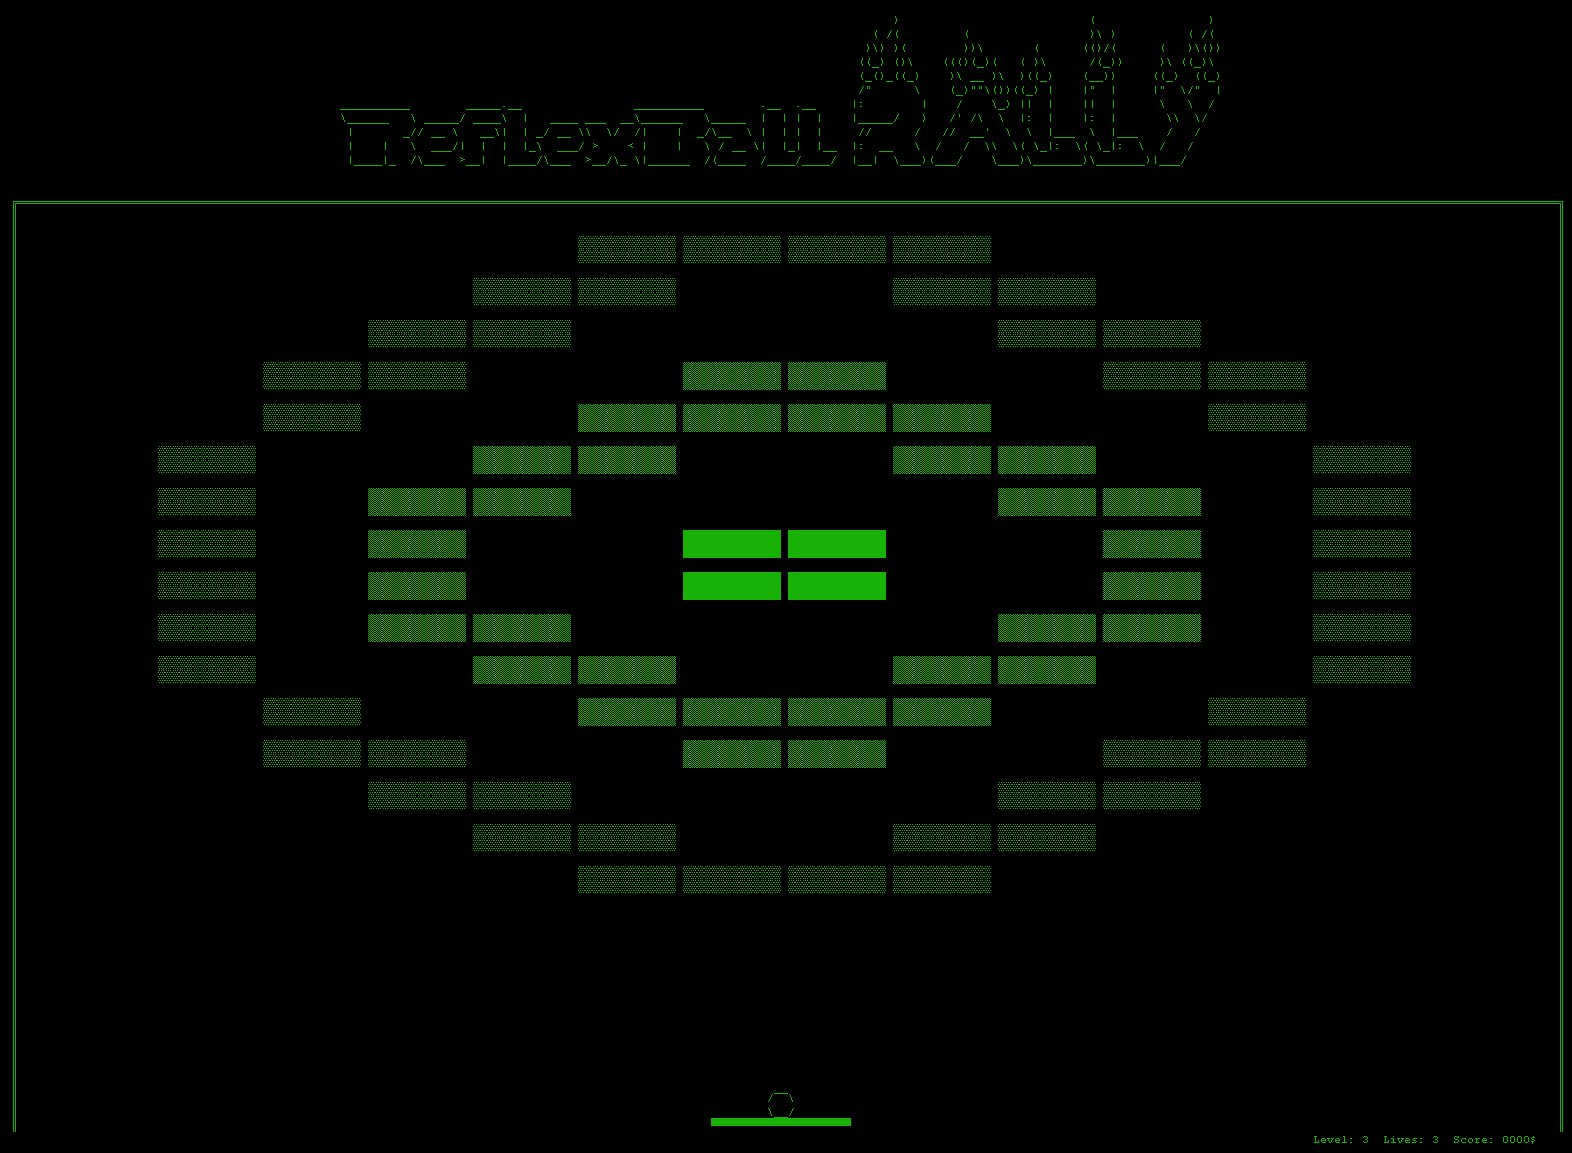
\includegraphics[width=\linewidth]{figs/screenshots/level3.png}
\caption{Level 3}
\label{fig:level3}
\end{minipage}\hfill
\begin{minipage}[b]{0.32\textwidth}
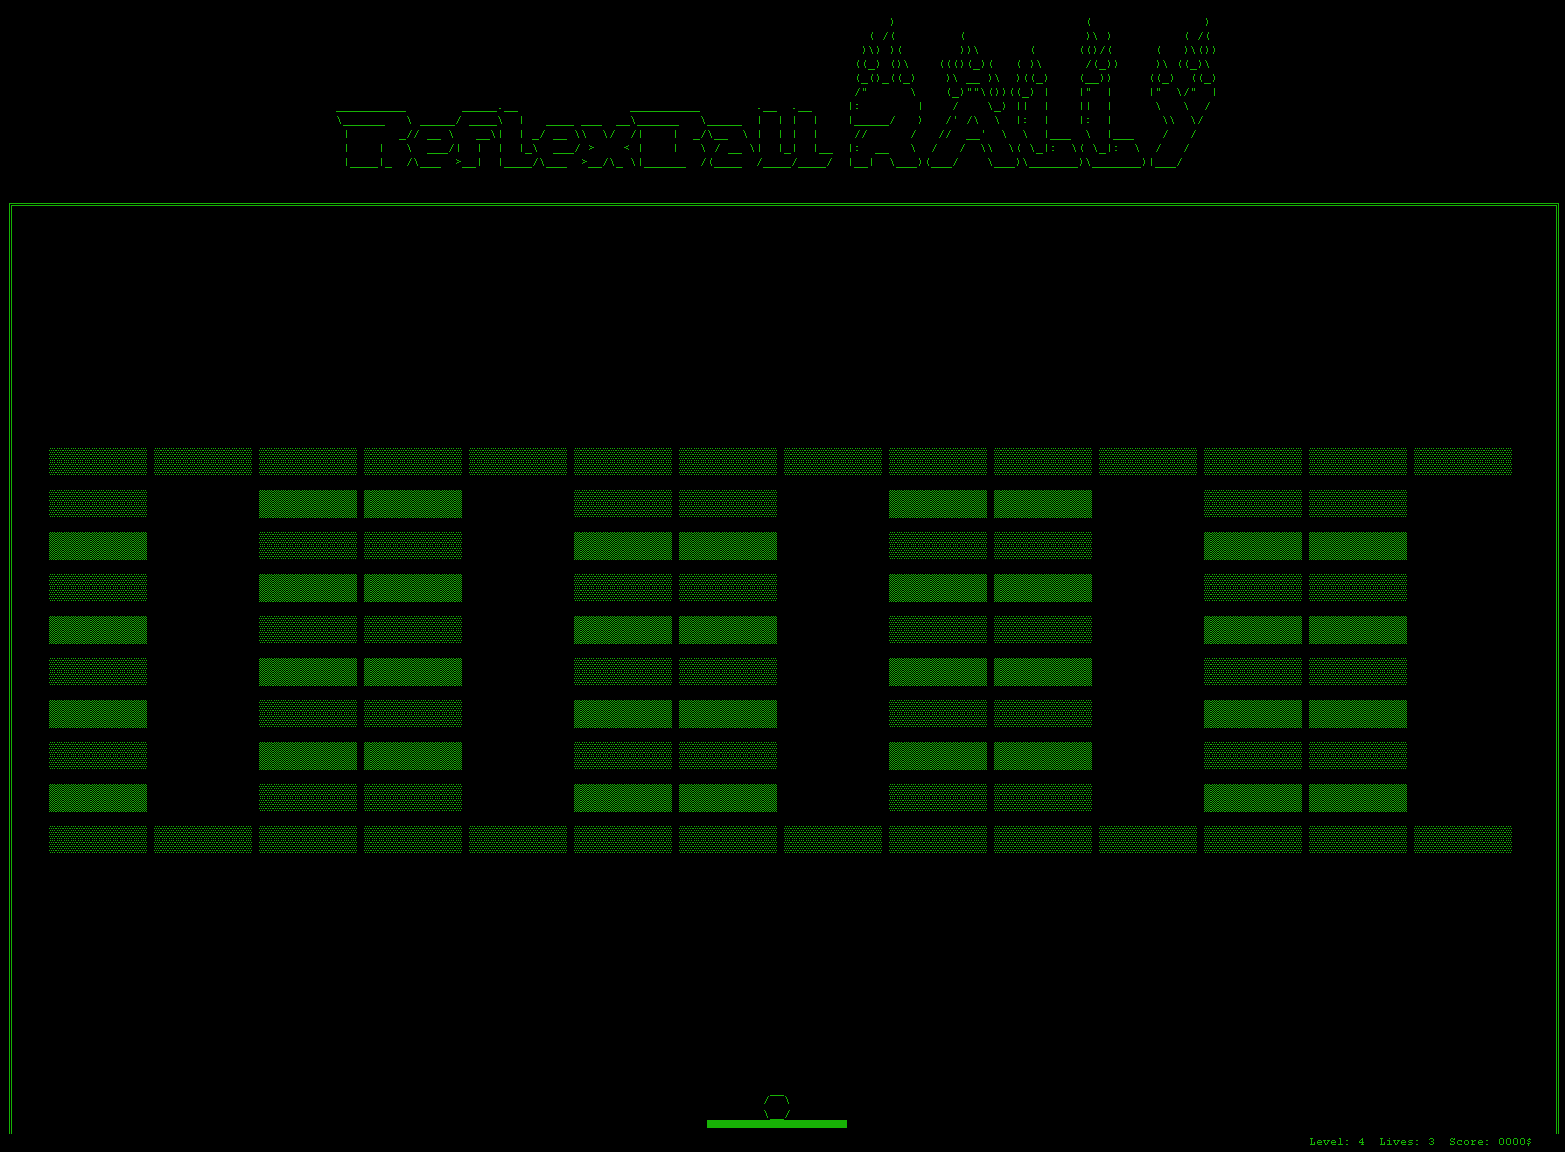
\includegraphics[width=\linewidth]{figs/screenshots/level4.png}
\caption{Level 4}
\label{fig:level4}
\end{minipage}\hfill
\begin{minipage}[b]{0.32\textwidth}
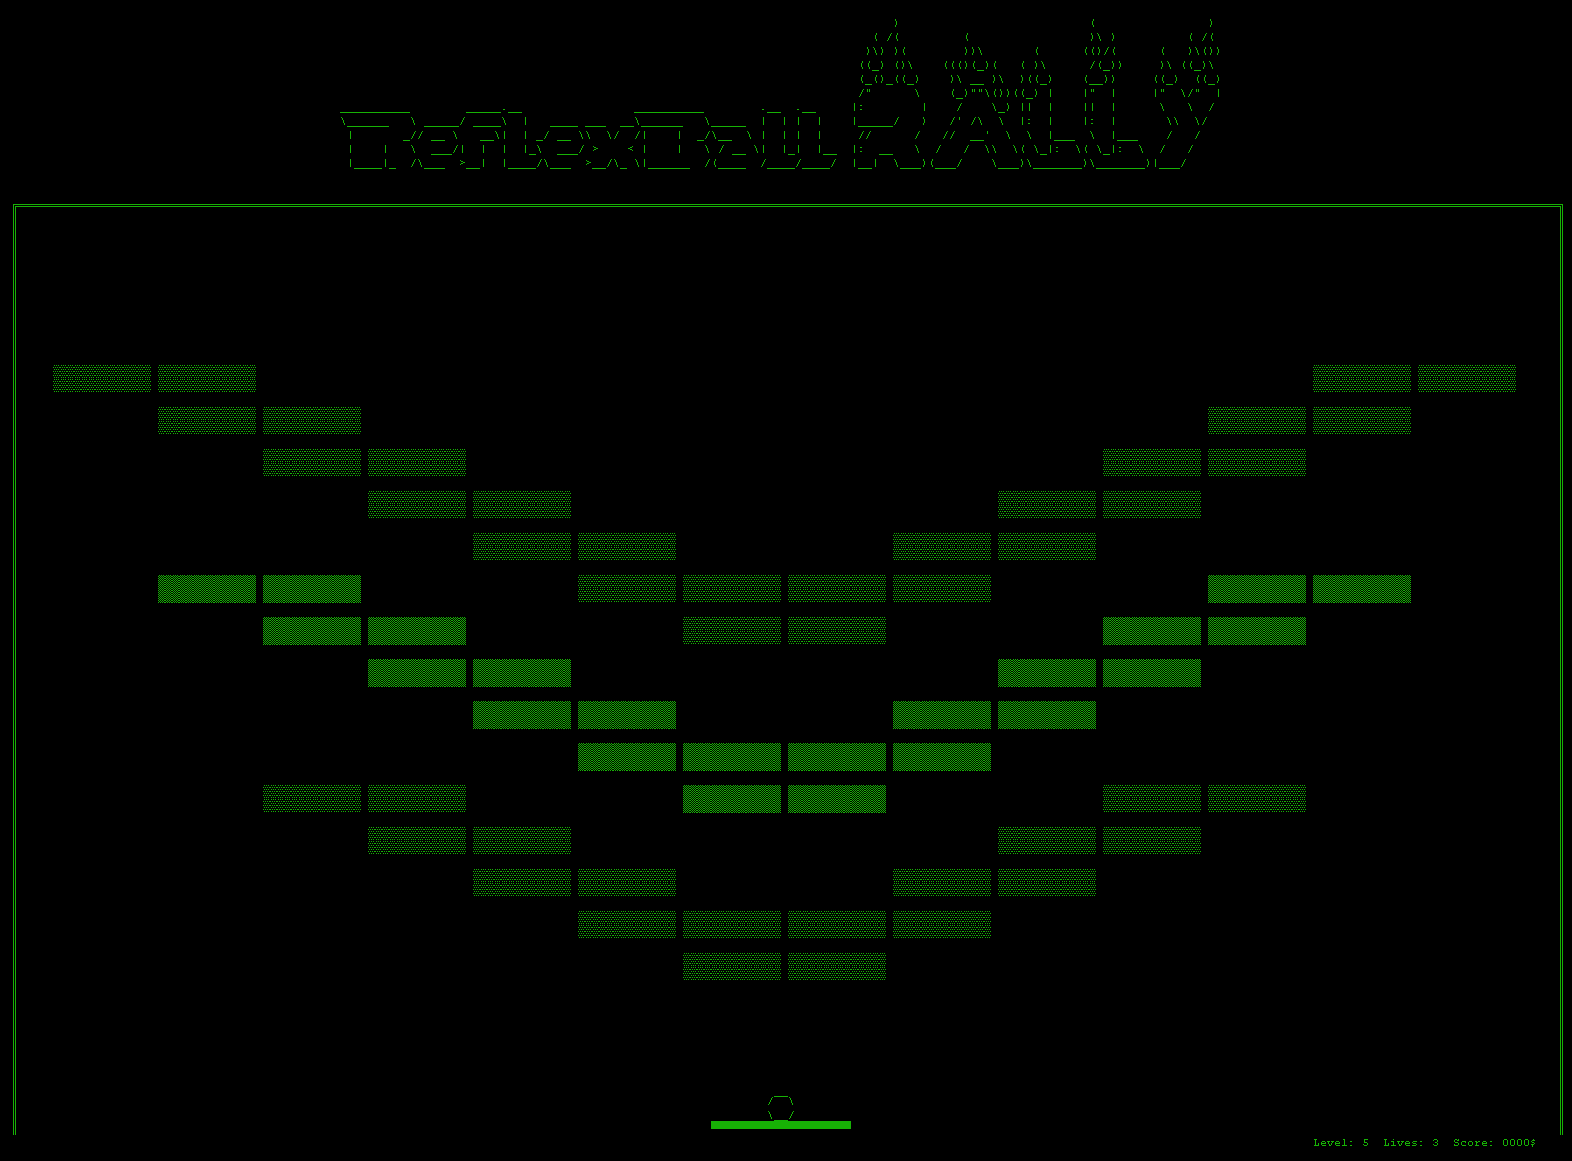
\includegraphics[width=\linewidth]{figs/screenshots/level5.png}
\caption{Level 5}
\label{fig:level5}
\end{minipage}\hfill
\begin{minipage}[b]{0.32\textwidth}
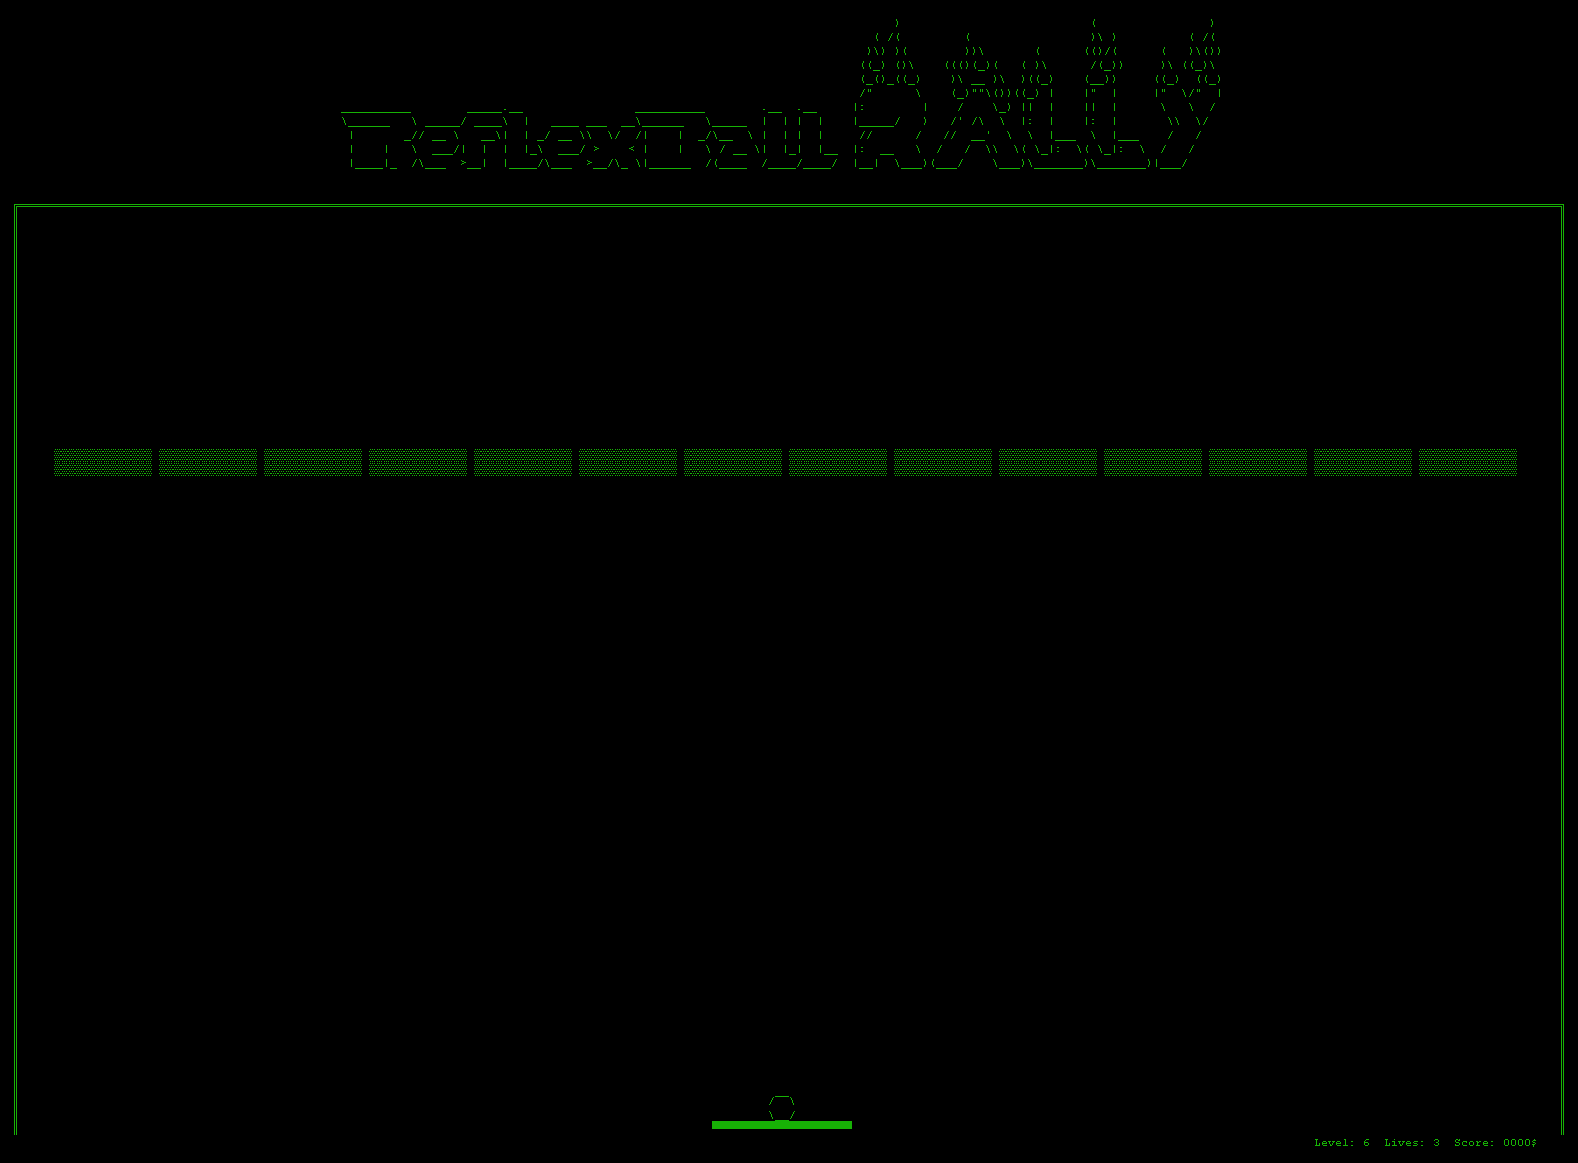
\includegraphics[width=\linewidth]{figs/screenshots/level6.png}
\caption{Level 6}
\label{fig:level6}
\end{minipage}\hfill
\end{figure}

Hvis man taber spillet vises "Game Over!" skrevet med ASCII art, samt 1 tilfældig ud af 8 forskellige undertitler. Figur \ref{fig:gameover_2} viser et screenshot af dette. \\

\begin{figure}[h!]
\centering

\includegraphics[scale=0.25]{figs/screenshots/gameover_crop.png}
\caption{Eksempel på screenshot game over tekst}
\label{fig:gameover_2}
\end{figure}

Hvis man vinder spillet på easy, medium eller hard vises et screenshot magen til figur \ref{fig:won_normal_2}, hvis man derimod vinder spillet på sværhedsgraden Chuck Norris vises et billedet som ses på figur \ref{fig:won_chuck}.

\begin{figure}[h!]
\begin{minipage}[b]{0.49\textwidth}

\includegraphics[width=\linewidth]{figs/screenshots/won_normal.png}
\caption{Screenshot ved gennemførsel af spillet}
\label{fig:won_normal_2}
\end{minipage}\hfill
\begin{minipage}[b]{0.49\textwidth}

\includegraphics[width=\linewidth]{figs/screenshots/won_chuck_crop.png}
\caption{Screenshot ved gennemførsel af spillet i Chuck Norris mode}
\label{fig:won_chuck}
\end{minipage}\hfill
\end{figure}